\section{二阶方法}
\label{sec:mfo-second-order}

一阶方法在贯穿例上每轮把误差减半，曲率矩阵的条件数变大时会更慢。切空间里的曲率信息能否换来一个更准确的步？接下来要弄清：这个线性子问题怎样写出，什么时候它的解值得采用？

需要分清三个判断，它们常常被混为一谈。模型非退化说的是线性子问题有唯一解，方向下降说的是这个解确实使目标减小，局部极小说的是所趋向的点是极小点。表~\ref{tab:mfo-three-judgments}用第~\ref{chap:second-order-methods}章的语言把它们并列。

\begin{BookInlineTable}
 \centering
 \caption{曲率算子的三种判断，$\bm{H}$是当前点的黎曼Hessian。}
 \label{tab:mfo-three-judgments}
 \begin{tabular}{lll}
  \toprule
  判断 & 条件 & 不保证什么\\
  \midrule
  模型非退化 & $\bm{H}$可逆 & 解是下降方向\\
  方向下降 & $\bm{H}$在切空间上正定即可 & 趋向极小点的全局性\\
  局部极小 & 驻点处$\bm{H}$正定 & 全局极小\\
  \bottomrule
 \end{tabular}
\end{BookInlineTable}

\subsection{黎曼Newton法}
\label{sec:mfo-newton}

\paragraph{主要思想}
由第~\ref{sec:mfo-pullback}节，模型~\eqref{eq:mfo-model}是拉回函数在零点的二阶近似。令模型的梯度为零，就得到切空间内的线性方程，\term{黎曼Newton法}（Riemannian Newton method）解这个方程再回缩：
\begin{equation}
 \operatorname{Hess}f(\bm{x}^{(t)})[\bm{v}^{(t)}]=-\bm{g}^{(t)},\quad\bm{v}^{(t)}\in T_{\bm{x}^{(t)}}M,
 \qquad
 \bm{x}^{(t+1)}=R_{\bm{x}^{(t)}}(\bm{v}^{(t)}).
 \label{eq:mfo-newton}
\end{equation}
未知量被限制在切空间中，这正是与欧氏Newton法不同的地方。方程的维数是$\dim M$，而不是环境空间的维数。

球面Rayleigh商上这个方程可以显式解出。由式~\eqref{eq:mfo-rayleigh-grad}和式~\eqref{eq:mfo-rayleigh-hess}，方程写成
\[
 \bm{P}_{\bm{x}}\bigl(\bm{A}\bm{v}\bigr)-q\bm{v}=-\bigl(\bm{A}\bm{x}-q\bm{x}\bigr),\qquad\bm{v}\perp\bm{x}.
\]

去掉投影时要补上一个沿$\bm{x}$的未知倍数$\lambda$。设$\bm{A}-q\bm{I}$可逆，移项后得到
\[
 (\bm{A}-q\bm{I})(\bm{x}+\bm{v})=\lambda\bm{x},\qquad
 \bm{x}+\bm{v}=\lambda(\bm{A}-q\bm{I})^{-1}\bm{x}.
\]

再用$\bm{x}^\top\bm{v}=0$确定$\lambda$，也就是$\bm{x}^\top(\bm{x}+\bm{v})=1$。于是
\begin{equation}
 \bm{x}+\bm{v}=\frac{(\bm{A}-q\bm{I})^{-1}\bm{x}}{\bm{x}^\top(\bm{A}-q\bm{I})^{-1}\bm{x}}.
 \label{eq:mfo-newton-closed}
\end{equation}

归一化之后分母的倍数消失，Newton迭代成为
\begin{equation}
 \bm{x}^{(t+1)}=\pm\frac{(\bm{A}-q^{(t)}\bm{I})^{-1}\bm{x}^{(t)}}{\bigl\lVert(\bm{A}-q^{(t)}\bm{I})^{-1}\bm{x}^{(t)}\bigr\rVert_2},
 \label{eq:mfo-rqi}
\end{equation}
符号由式~\eqref{eq:mfo-newton-closed}决定。这就是经典的Rayleigh商迭代。一个特征值算法，原来是球面上的Newton法加归一化回缩。

\needspace{6\baselineskip}
\paragraph{变量}
\begin{itemize}
 \item $\bm{x}^{(t)}$：球面上的当前点；$q^{(t)}$：Rayleigh商的取值。
 \item $\bm{z}=(\bm{A}-q^{(t)}\bm{I})^{-1}\bm{x}^{(t)}$：三维向量。
 \item $\lambda=1/(\bm{x}^{(t)\top}\bm{z})$：标量，由切向条件确定。
 \item $\bm{v}^{(t)}=\lambda\bm{z}-\bm{x}^{(t)}$：Newton步，切于$\bm{x}^{(t)}$。
\end{itemize}

\paragraph{初始化}
这里换一个更靠近解的起点，理由在后面解释。例中取
\[
 \bm{x}^{(0)}=\frac19(8,4,1)^\top,\qquad q^{(0)}=\frac{64+32+4}{81}=\frac{100}{81}.
\]
停止条件取$\lVert\bm{g}^{(t)}\rVert_2\leq10^{-6}$。

\needspace{6\baselineskip}
\paragraph{每轮更新}
\begin{enumerate}
 \item 计算$\bm{z}$。例中第$0$轮
 \[
  \bm{A}-q^{(0)}\bm{I}=\frac{1}{81}\operatorname{diag}(-19,62,224),
 \]
 所以
 \[
  \bm{z}=\Bigl(-\frac{72}{19},\ \frac{18}{31},\ \frac{9}{224}\Bigr)^\top\approx(-3.7895,\ 0.5806,\ 0.0402)^\top.
 \]

 \item 计算$\lambda$。例中$\bm{x}^{(0)\top}\bm{z}\approx-3.1058$，所以$\lambda\approx-0.3220$。

 \item 由式~\eqref{eq:mfo-newton-closed}得到$\bm{x}+\bm{v}$，由$\bm{v}=\lambda\bm{z}-\bm{x}$读出Newton步。例中
 \[
  \begin{gathered}
  \bm{x}^{(0)}+\bm{v}^{(0)}\approx(1.2201,-0.1870,-0.0129)^\top,\\
  \bm{v}^{(0)}\approx(0.3312,-0.6314,-0.1241)^\top.
  \end{gathered}
 \]

 \item 回缩。例中$\bm{x}^{(1)}\approx(0.9884,-0.1515,-0.0105)^\top$，$\lVert\bm{g}^{(1)}\rVert_2\approx0.1529$。
\end{enumerate}

继续迭代得到表~\ref{tab:mfo-newton-run}。第$3$轮满足停止条件，最终得到$\bm{x}^{(3)}\approx\bm{e}_1$，只用了三次线性方程的求解。

\begin{BookInlineTable}
 \centering
 \caption{从$(8,4,1)^\top/9$出发的黎曼Newton法。最后一列是切空间上$\bm{H}^{(t)}$的特征值。}
 \label{tab:mfo-newton-run}
 \begin{tabular}{lllll}
  \toprule
  $t$ & $\bm{x}^{(t)}$ & $q^{(t)}$ & $\lVert\bm{g}^{(t)}\rVert_2$ & $\bm{H}^{(t)}$的特征值\\
  \midrule
  $0$ & $(0.8889,0.4444,0.1111)$ & $1.2346$ & $0.5036$ & $0.5645,\ 2.7318$\\
  $1$ & $(0.9884,-0.1515,-0.0105)$ & $1.0233$ & $0.1529$ & $0.9538,\ 2.9764$\\
  $2$ & $(1.0000,0.0037,0.0001)$ & $1.0000$ & $3.66\times10^{-3}$ & $1.0000,\ 3.0000$\\
  $3$ & $(1.0000,0.0000,0.0000)$ & $1.0000$ & $4.87\times10^{-8}$ & $1.0000,\ 3.0000$\\
  \bottomrule
 \end{tabular}
\end{BookInlineTable}

\paragraph{局部收敛}
表中的梯度范数几乎是按立方在减小：$0.1529^3\approx3.6\times10^{-3}$，$(3.66\times10^{-3})^3\approx4.9\times10^{-8}$。一般情形的局部结论是平方收敛，这里的立方来自Rayleigh商的特殊结构。

一般结论是：设$\bm{x}^\star$是驻点，$\operatorname{Hess}f(\bm{x}^\star)$可逆，$f$足够光滑，$R$是光滑回缩，则存在$\bm{x}^\star$的邻域，从其中出发的迭代~\eqref{eq:mfo-newton}收敛到$\bm{x}^\star$，至少是平方速度。

严格证明要把迭代写进一张局部坐标图，再逐项控制回缩与坐标化带来的误差，篇幅较长，读者可查阅专门讨论流形优化的著作\scite{math-boumal2023optimization}。机制是这样的：第~\ref{sec:mfo-pullback}节表明，拉回Hessian与黎曼Hessian之差正比于$\lVert\operatorname{grad}f\rVert_2$，在解附近这个差与误差同阶，而一阶量的误差对Newton法只产生平方量级的后果。所以这里任何光滑回缩都行，不必是二阶回缩。

立方的来历可以直接算出。设$\bm{x}=\cos e\,\bm{e}_1+\sin e\,\bm{u}$，$\bm{u}$是$\bm{A}$的另一单位特征向量，特征值$\lambda_u$。Rayleigh商的误差是二阶的：
\[
 q-\lambda_1=(\lambda_u-\lambda_1)\sin^2e.
\]

$(\bm{A}-q\bm{I})^{-1}$把$\bm{e}_1$分量放大$1/(\lambda_1-q)$倍，把$\bm{u}$分量放大$1/(\lambda_u-q)$倍。两个分量的比值给出新的夹角：
\[
 \tan e^{+}=\tan e\cdot\frac{\lvert\lambda_1-q\rvert}{\lvert\lambda_u-q\rvert}=\tan e\cdot\frac{\sin^2e}{\cos^2e}=\tan^3e.
\]
这里用了$\lambda_u-q=(\lambda_u-\lambda_1)\cos^2e$。当$\bm{x}$的误差主要在一个特征方向上时立方律是精确的，这解释了表中系数接近一。

图~\ref{fig:mfo-newton-rate}把这个速度与上一节的梯度下降放在同一张图上。

\begin{BookInlineFigure}
 \centering
 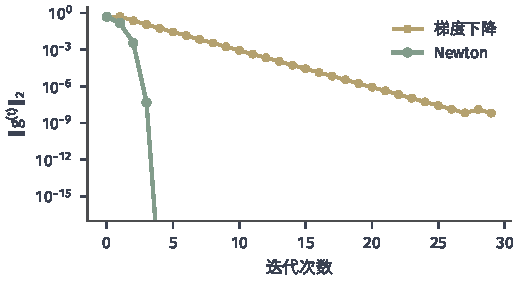
\includegraphics[width=88.0mm]{figures/05-optimization/06-constrained-optimization/matplotlib/mfo-newton-rate/figure.pdf}
 \caption{从同一起点$(8,4,1)^\top/9$出发的黎曼梯度范数。绿线是黎曼Newton法，黄线是回溯线搜索的梯度下降。}
 \label{fig:mfo-newton-rate}
\end{BookInlineFigure}

\paragraph{远离解时}
回到原来的起点$\bm{x}^{(0)}=\tfrac13(2,2,1)^\top$，就能看到为什么上面要换起点。在基$\bm{E}_1,\bm{E}_2$下，$\bm{g}$和$\bm{H}$的坐标表示可由$\bm{A}-q\bm{I}$（对角元为$-\tfrac79,\tfrac29,\tfrac{20}{9}$）算出：
\[
 \bm{g}=\begin{bmatrix}2/9\\-8/9\end{bmatrix},\qquad
 \bm{H}=\begin{bmatrix}1&-10/9\\-10/9&2/3\end{bmatrix},\qquad
 \det\bm{H}=-\frac{46}{81}.
\]
行列式为负，$\bm{H}$的特征值约为$-0.290$和$1.957$，这里模型非退化，但不正定。

解线性方程，得到Newton步的坐标
\[
 \bm{v}=-\bm{H}^{-1}\bm{g}=-\Bigl(\frac{34}{23},\ \frac{26}{23}\Bigr)^\top.
\]

检查方向导数，它是正的：
\[
 \langle\bm{g},\bm{v}\rangle=-\frac29\cdot\frac{34}{23}+\frac89\cdot\frac{26}{23}=\frac{140}{207}>0.
\]
Newton步是上升方向。回缩后的点约为$(-0.274,0.960,0.048)^\top$，目标值从$0.889$升到$0.965$，这个点靠近鞍点$\bm{e}_2$。

这个现象并非偶然。Newton法寻找的是驻点，它对极小点、鞍点和极大点一视同仁。图~\ref{fig:mfo-newton-basin}标出未加保护的Rayleigh商迭代从球面上各点出发时的去向，起点$\bm{x}^{(0)}$恰好落在通往$\bm{e}_2$的区域。

\begin{BookInlineFigure}
 \centering
 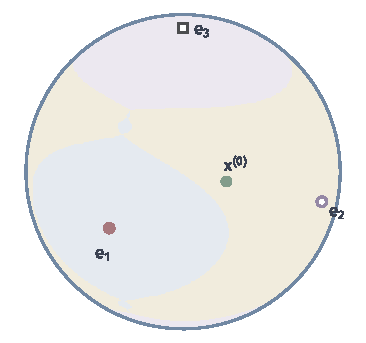
\includegraphics[width=62.0mm]{figures/05-optimization/06-constrained-optimization/matplotlib/mfo-newton-basin/figure.pdf}
 \caption{未加保护的黎曼Newton迭代的去向。每个点的底色表示从该点出发$40$步后趋向哪一对特征向量：浅蓝趋向$\pm\bm{e}_1$，浅黄趋向$\pm\bm{e}_2$，浅紫趋向$\pm\bm{e}_3$。绿点是起点$\bm{x}^{(0)}$，它落在浅黄区域。}
 \label{fig:mfo-newton-basin}
\end{BookInlineFigure}

\subsection{阻尼与非精确求解}
\label{sec:mfo-damped-inexact}

Newton步需要两层保护：方向要下降，步长要合适。规模大的时候还有第三个问题，线性方程不能精确求解。这三件事的思想都来自第~\ref{chap:second-order-methods}章，本节只说明在切空间上有什么变化。

\paragraph{修正曲率}
若$\bm{H}$在切空间上正定，Newton步是下降方向，因为
\[
 \langle\bm{g},\bm{v}\rangle=-\langle\bm{v},\bm{H}[\bm{v}]\rangle<0.
\]
否则就把$\bm{H}$换成$\bm{H}+\tau\bm{I}$，$\tau>0$大到足以使它在切空间上正定。这里的$\bm{I}$是切空间上的恒等算子。

在贯穿例的起点取$\tau=1$，修正后的特征值约为$0.710$和$2.957$，正定。解线性方程得到
\[
 \bm{v}=-(\bm{H}+\bm{I})^{-1}\bm{g}=\Bigl(\frac{5}{17},\ \frac{62}{85}\Bigr)^\top\approx(0.2941,\ 0.7294)^\top.
\]

方向导数约为$-0.583$，确实下降。用$c_1=\tfrac14$做回缩线搜索，试探$\alpha=1$，得到
\[
 R_{\bm{x}^{(0)}}(\bm{v})\approx(0.9833,0.1788,0.0339)^\top,\qquad f\approx0.5177.
\]
下降约$0.371$，超过要求的$0.146$，接受。这一步的目标值比梯度下降第$1$轮的$0.6468$小得多。

Armijo线搜索在这里同样要针对回缩后的点。切向方向下降只保证步足够短时有效，与第~\ref{sec:mfo-rgd}节的道理相同。

\paragraph{用Hessian--向量乘积代替形成矩阵}
当$\dim M$很大时，不可能写出$\bm{H}$的矩阵。Rayleigh商的式~\eqref{eq:mfo-rayleigh-hess}告诉我们，算$\bm{H}[\bm{v}]$只需要一次$\bm{A}$乘向量和一次投影，所以可以用线性共轭梯度法迭代求解式~\eqref{eq:mfo-newton}。

这里的“共轭梯度”要与第~\ref{sec:mfo-rcg}节区分开，表~\ref{tab:mfo-cg-compare}列出区别。内层CG全程在同一个切空间中，解一个线性方程，不需要回缩和搬运。

\begin{BookInlineTable}
 \centering
 \caption{两种共轭梯度。}
 \label{tab:mfo-cg-compare}
 \begin{tabular}{lll}
  \toprule
  & 内层线性CG & 黎曼共轭梯度\\
  \midrule
  解决的问题 & 切空间内的线性方程 & 流形上的非线性优化\\
  所在空间 & 固定的$T_{\bm{x}}M$ & 每轮更换切空间\\
  回缩与搬运 & 不需要 & 每轮都需要\\
  曲率使用 & Hessian--向量乘积 & 不使用\\
  \bottomrule
 \end{tabular}
\end{BookInlineTable}

\paragraph{按切空间的残差设定精度}
线性方程不必解得太准。切空间内的残差是$\bm{r}=\bm{H}[\bm{v}]+\bm{g}$，内层在下述条件满足时停止：
\begin{equation}
 \lVert\bm{r}\rVert_2\leq\eta^{(t)}\lVert\bm{g}^{(t)}\rVert_2.
 \label{eq:mfo-forcing}
\end{equation}
第~\ref{chap:second-order-methods}章的结论在这里同样适用：固定的$\eta<1$一般只给出线性收敛，$\eta^{(t)}\to0$给出超线性收敛，$\eta^{(t)}=O(\lVert\bm{g}^{(t)}\rVert_2)$在解附近恢复平方收敛。

图~\ref{fig:mfo-inexact-newton}是$n=500$的实验。三种规则的总Hessian--向量乘积数分别约为$815$、$815$、$855$，差别很小，外层迭代数分别为$60$、$43$、$41$。收益集中在收尾阶段：远离解时三条曲线几乎重合，此时的工作量由全局下降决定，更严的容差也帮不上忙。

\begin{BookInlineFigure}
 \centering
 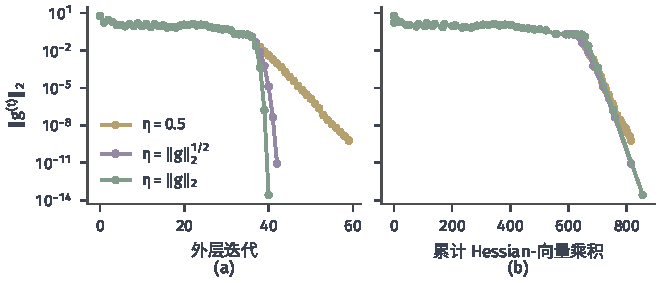
\includegraphics[width=112.0mm]{figures/05-optimization/06-constrained-optimization/matplotlib/mfo-inexact-newton/figure.pdf}
 \caption{$n=500$，$\bm{A}$的特征值在$1$到$100$之间等距，随机起点固定，球面上的Newton--CG加回溯线搜索。内层容差分别取$\eta=0.5$（黄）、$\min\{0.5,\lVert\bm{g}\rVert_2^{1/2}\}$（紫）、$\min\{0.5,\lVert\bm{g}\rVert_2\}$（绿）。(a)~按外层迭代。(b)~按累计Hessian--向量乘积。}
 \label{fig:mfo-inexact-newton}
\end{BookInlineFigure}

\paragraph{负曲率与切向数值误差}
内层CG计算$\langle\bm{d},\bm{H}[\bm{d}]\rangle$时，若它不大于零，说明遇到了负曲率方向，线性方程的解不再是模型的极小点。这时要停止CG：若是第一步，取负梯度方向；否则返回当前的$\bm{v}$，它仍是下降方向。

另一个要小心的是舍入误差。理论上$\bm{H}$把切空间映到切空间，CG的向量始终是切向的。实际计算中会累积沿法向的分量，维数高、CG步数多时尤其明显。常用做法是每隔若干步把$\bm{v}$、$\bm{r}$和$\bm{d}$重新投影到切空间。
